%% ****** Start of file template.aps ****** %
%%
%%
%%   This file is part of the APS files in the REVTeX 4 distribution.
%%   Version 4.0 of REVTeX, August 2001
%%
%%
%%   Copyright (c) 2001 The American Physical Society.
%%
%%   See the REVTeX 4 README file for restrictions and more information.
%%
%
% This is a template for producing manuscripts for use with REVTEX 4.0
% Copy this file to another name and then work on that file.
% That way, you always have this original template file to use.
%
% Group addresses by affiliation; use superscriptaddress for long
% author lists, or if there are many overlapping affiliations.
% For Phys. Rev. appearance, change preprint to twocolumn.
% Choose pra, prb, prc, prd, pre, prl, prstab, or rmp for journal
%  Add 'draft' option to mark overfull boxes with black boxes
%  Add 'showpacs' option to make PACS codes appear
%  Add 'showkeys' option to make keywords appear
\documentclass{revtex4}
%\documentclass[aps,prl,preprint,superscriptaddress]{revtex4}
%\documentclass[aps,prl,twocolumn,groupedaddress]{revtex4}
\usepackage[dvipdf]{graphicx}
%\usepackage{dcolumn}

% You should use BibTeX and apsrev.bst for references
% Choosing a journal automatically selects the correct APS
% BibTeX style file (bst file), so only uncomment the line
% below if necessary.
%\bibliographystyle{apsrev}

\begin{document}

% Use the \preprint command to place your local institutional report
% number in the upper righthand corner of the title page in preprint mode.
% Multiple \preprint commands are allowed.
% Use the 'preprintnumbers' class option to override journal defaults
% to display numbers if necessary
%\preprint{}

%Title of paper
\title{Determination of the Normal Modes of a Pair of Coupled Pendulums}

% repeat the \author .. \affiliation  etc. as needed
% \email, \thanks, \homepage, \altaffiliation all apply to the current
% author. Explanatory text should go in the []'s, actual e-mail
% address or url should go in the {}'s for \email and \homepage.
% Please use the appropriate macro foreach each type of information

% \affiliation command applies to all authors since the last
% \affiliation command. The \affiliation command should follow the
% other information
% \affiliation can be followed by \email, \homepage, \thanks as well.
\author{Physics 2501: Mechanics and Electromagnetism Laboratory}
%\homepage[]{Your web page}
%\thanks{}
%\altaffiliation{}
\affiliation{Dept. of Physics, University of Connecticut}
%\author{R.T. Jones}
%\affiliation{University of Connecticut}

%Collaboration name if desired (requires use of superscriptaddress
%option in \documentclass). \noaffiliation is required (may also be
%used with the \author command).
%\collaboration can be followed by \email, \homepage, \thanks as well.
%\collaboration{}
%\noaffiliation

\date{\today}

%\begin{abstract}
% insert abstract here
%\end{abstract}

% insert suggested PACS numbers in braces on next line
%\pacs{}
% insert suggested keywords - APS authors don't need to do this
%\keywords{}

%\setlength{\topmargin}{0in}

%\maketitle must follow title, authors, abstract, \pacs, and \keywords
\maketitle

% body of paper here - Use proper section commands
% References should be done using the \cite, \ref, and \label commands

%% The normal text is displayed in two-column format, but special
%% sections spanning both columns can be inserted within the page
%% format so that long equations can be displayed. Use
%% sparingly.
%%\begin{widetext}
%% put long equation here
%%\end{widetext}
%
%% figures should be put into the text as floats.
%% Use the graphics or graphicx packages (distributed with LaTeX2e)
%% and the \includegraphics macro defined in those packages.
%% See the LaTeX Graphics Companion by Michel Goosens, Sebastian Rahtz,
%% and Frank Mittelbach for instance.
%%
%% Here is an example of the general form of a figure:
%% Fill in the caption in the braces of the \caption{} command. Put the label
%% that you will use with \ref{} command in the braces of the \label{} command.
%% Use the figure* environment if the figure should span across the
%% entire page. There is no need to do explicit centering.
%
%%\begin{turnpage}
%% Surround figure environment with turnpage environment for landscape
%% figure
%% \begin{turnpage}
%% \begin{figure}
%% \includegraphics{}%
%% \caption{\label{}}
%% \end{figure}
%% \end{turnpage}
%
%% tables should appear as floats within the text
%%
%% Here is an example of the general form of a table:
%% Fill in the caption in the braces of the \caption{} command. Put the label
%% that you will use with \ref{} command in the braces of the \label{} command.
%% Insert the column specifiers (l, r, c, d, etc.) in the empty braces of the
%% \begin{tabular}{} command.
%% The ruledtabular enviroment adds doubled rules to table and sets a
%% reasonable default table settings.
%% Use the table* environment to get a full-width table in two-column
%% Add \usepackage{longtable} and the longtable (or longtable*}
%% environment for nicely formatted long tables. Or use the the [H]
%% placement option to break a long table (with less control than 
%% in longtable).
%
%
%% Surround table environment with turnpage environment for landscape
%% table
%% \begin{turnpage}
%% \begin{table}
%% \caption{\label{}}
%% \begin{ruledtabular}
%% \begin{tabular}{}
%% \end{tabular}
%% \end{ruledtabular}
%% \end{table}
%% \end{turnpage}
%
%% Specify following sections are appendices. Use \appendix* if there
%% only one appendix.
%%\appendix
%%\section{}
%

\section{Introduction}

It is a fact beyond doubt that the simple harmonic oscillator is the most
frequently used model in all of physics.  Applicable to both to large-scale
structures like aircraft and bridges, and to smaller structures like
atoms and nuclei, this simple model gives important insight into the
behavior of even the most complicated systems when their dynamics are
governed by small departures from equilibrium.  In its simplest form,
the model predicts that a coordinate describing a degree of freedom, such
as a displacement or a twist, will undergo sinusoidal oscillations at a
unique frequency that is characteristic of the system and independent of
the amplitude of the oscillations.  This model can be extended to
multi-body systems, such as atoms in a crystal lattice, by starting with
a simple picture of multiple independent oscillators, and then introduce
a way for them to weakly perturb one another. In this experiment, you
will investigate what effects are produced on a pair of identical
independent pendulum oscillators when a weak coupling in introduced
between them in the form of a spring.

\begin{figure}
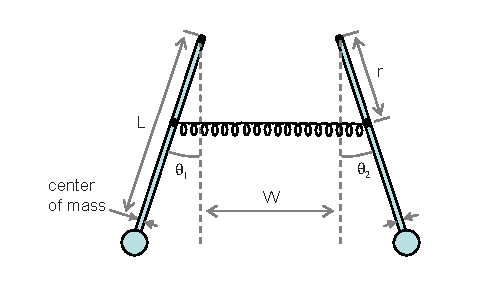
\includegraphics[width=10cm]{2pendulumsfig.eps}
\caption{\label{2pendulumsfig} 
The initial setup consists of two similar pendulums of masses $M_1$
and $M_2$ suspended so that they oscillate freely about pivots on their
top end.  The center of mass without the spring attached is a distance
$L_1 \simeq L_2$ from the pivot.  Later, a spring with spring constant
$K$ is attached to each pendulum a distance $r_1\simeq r_2$ from the pivots.
The apparatus accommodates several different choices of values for $r$.}
\end{figure}

Consider the two identical pendulum bobs displayed in
Fig.~\ref{2pendulumsfig}. Without the coupling spring,
the small-amplitude motion of either pendulum is described by
\begin{equation}
I\frac{d^2\theta}{dt^2} = -MgL\theta
\end{equation}
where $I$ is the moment of inertia about the pivot point and $L$ is the
distance from the pivot to the center of mass. The resulting motion is
simple harmonic,
\begin{equation}
\theta(t) = A \sin(\omega t + \delta)
\end{equation}
where the angular frequency is
\begin{equation}
\omega = \sqrt{\frac{MgL}{I}} \label{eq:omegadef}
\end{equation}
and the oscillation period is
\begin{equation}
\tau = \frac{2\pi}{\omega} \label{eq:omega2tau}
\end{equation}

Now consider the situation in which the two pendulums are coupled together
by a spring whose spring constant is $K$ and whose unstretched length is
$S$.  In the small-angle approximation, the spring is stretched by a
distance
\begin{equation}
x = W-S+r_1\theta_1+r_2\theta_2
\end{equation}
The angular equations of small-amplitude motion for the two pendulums,
modified to include the additional torque produced by the action of the
spring, are
\begin{eqnarray}
I_1\frac{d^2\theta_1}{dt^2} &=& -M_1gL_1\theta_1 - Kr_1x \nonumber \\
    &=& -(M_1gL_1+Kr_1^2)\theta_1 - Kr_1^2\theta_2 - Kr_1(W-S)
    \label{eq:eom1}\\
I_2\frac{d^2\theta_2}{dt^2} &=& -M_2gL_2\theta_2 - Kr_2x \nonumber \\
    &=& -(M_2gL_2+Kr_2^2)\theta_2 - Kr_2^2\theta_1 - Kr_2(W-S)
    \label{eq:eom2}
\end{eqnarray}

The equilibrium angles of the pendulums are no longer exactly vertical
due to the torques from the spring.  The equilibrium angular displacements
$\theta_{10}$ and $\theta_{20}$ are found by solving simultaneous
equations \ref{eq:eom1} and \ref{eq:eom2} for the static case where the
left-hand sides are zero.  In the special case where the two pendulums are
identical, they both have the same equilibrium displacement
\begin{equation}
\theta_{10} = \theta_{20} = -\frac{Kr(W-S)}{MgL+2Kr^2}
\end{equation}
but this assumption is not essential.  In the more general case, one
can always define new angles that are measured as angular displacements
from equilibrium where ever it is, as
\begin{eqnarray}
\phi_1 &=& \theta_1-\theta_{10} \nonumber \\
\phi_2 &=& \theta_2-\theta_{20} \nonumber
\end{eqnarray}
whose equations of motions are the same as those of $\theta_1$ and
$\theta_2$ except that they are missing the constant term on the right
hand side.  It is illuminating to write these equations in matrix form,
as
\begin{equation}
{\mathbf I} \frac{d^2}{dt^2} \Phi = -{\mathbf R} \Phi
\end{equation}
where
\[ {\mathbf I} = \left(
\begin{array}{cc}
I_1 & 0 \\
0 & I_2
\end{array}
\right) \]
\[ {\mathbf R} = \left(
\begin{array}{cc}
M_1L_1g+Kr_1^2 & Kr_1r_2 \vspace*{2mm} \\
Kr_1r_2 & M_2L_2g+Kr_2^2
\end{array}
\right) \]
\[ \Phi = \left[
\begin{array}{cc}
\phi_1 \\
\phi_2
\end{array}
\right] \]
Casting this in the form of the simple harmonic oscillator equation
of motion leads to 
\begin{equation}
\frac{d^2}{dt^2} \Phi = -{\mathbf M} \Phi \label{eq:eom4phi}
\end{equation}
where
\begin{equation}
{\mathbf M} = \left(
\begin{array}{cc}
\omega_1^2+\omega_3^2 & \omega_3^2r_2/r_1 \vspace*{2mm} \\
\omega_4^2r_1/r_2 & \omega_2^2+\omega_4^2
\end{array}
\right)
\end{equation}
where $\omega_1$ and $\omega_2$ are the natural frequencies of pendulums
1 and 2 with no spring attached,
\begin{eqnarray}
\omega_1 &=& \sqrt{\frac{M_1L_1g}{I_1}} \label{eq:omega1} \\
\omega_2 &=& \sqrt{\frac{M_2L_2g}{I_2}} \label{eq:omega2}
\end{eqnarray}
and $\omega_3$ and $\omega_4$ are defined as
\begin{eqnarray}
\omega_3 &=& \sqrt{\frac{Kr_1^2}{I_1}} \label{eq:omega3} \\
\omega_4 &=& \sqrt{\frac{Kr_2^2}{I_2}} \label{eq:omega4}
\end{eqnarray}

To solve this differential equation, first find the eigenvalues of
the matrix ${\mathbf M}$.  This $2\times 2$ matrix in general is expected
to possess two eigenvalues denoted here as $m_+$ and $m_-$, with the
corresponding eigenvectors denoted as $\Phi_+$ and $\Phi_-$.
\begin{equation}
{\mathbf M}\Phi_{\pm} = m_{\pm} \Phi_{\pm} \label{eq:eigeneq}
\end{equation}
Solving Eq.~\ref{eq:eigeneq} leads to the following characteristic
equation for the eigenvalues $m$,
\begin{eqnarray}
Am^2 + Bm + C &=& 0\hspace*{2mm}\mbox{, where} \\
A &=& 1 \nonumber \\
B &=& -(\omega_1^2+\omega_2^2+\omega_3^2+\omega_4^2 \nonumber) \\
C &=& (\omega_1^2+\omega_3^2)(\omega_2^2+\omega_4^2) - \omega_3^2\omega_4^2
\nonumber
\end{eqnarray}
with solutions
\begin{equation}
m_{\pm} = \frac{-B \pm \sqrt{B^2-4AC}}{2A} \label{eq:eigenvals}
\end{equation}
where $m_+$ indicates the solution obtained when taking the positive
root of the discriminant, and $m_-$ indicates the other solution.
Eq.~\ref{eq:eigenvals} is greatly simplified if one can assume
that the two pendulums have the same natural frequency when oscillating
freely without the spring attached.  In this case,
\begin{eqnarray}
m_- &=& \omega_0^2 \\
m_+ &=& \omega_0^2 +\omega_3^2+\omega_4^2
\end{eqnarray}
where $\omega_0\equiv \omega_1=\omega_2$.  This assumption makes no
difference conceptually, but it will be used from now on to simplify
the expressions.  Corresponding to these two eigenvalues are the
eigenvectors $\Phi_{\pm}$
\begin{eqnarray}
\Phi_- &=& \left(
\begin{array}{c}
1 \\
-\frac{r_1}{r_2}
\end{array}\right) \\
\Phi_+ &=& \left(
\begin{array}{c}
1 \\
\frac{\omega_4^2 r_1}{\omega_3^2 r_2}
\end{array}\right)
\end{eqnarray}
as is verified by substitution back into Eq.~\ref{eq:eigeneq}.

General solutions to the equations of motion in
Eq.~\ref{eq:eom4phi} are constructed out of arbitrary superpositions
of the these two eigenvalues and eigenvectors, as
\begin{equation}
\Phi(t) = a_-\Phi_-\sin(\omega_-t+\delta_-)
        + a_+\Phi_+\sin(\omega_+t+\delta_+) \label{eq:superp}
\end{equation}
where amplitudes $a_{\pm}$ and initial phases $\delta_{\pm}$ are
determined by the initial conditions of the motion.  Eq.~\ref{eq:eom4phi}
fixes the two oscillation frequencies at
\begin{eqnarray}
\omega_- &=& \sqrt{m_-} = \omega_0 \label{eq:omega-} \\
\omega_+ &=& \sqrt{m_+} = \sqrt{\omega_0^2+\omega_3^2+\omega_4^2}
\label{eq:omega+}
\end{eqnarray}

In this experiment we are particularly interested in the special case
where the two pendulums are nearly identical.  In this case $r_1=r_2$
and $\omega_3=\omega_4$, and the normal mode solutions become
\[
\Phi_- = \left(
\begin{array}{c}
1 \\ 
-1
\end{array}\right)\hspace*{5mm}
\mbox{and}\hspace*{5mm}
\Phi_+ = \left(
\begin{array}{c}
1 \\ 
1
\end{array}\right)\hspace*{2mm}.
\]
The first case above corresponds to the two pendulums swinging left
and right at the same time (the negative sign comes about because of
the opposite convention used when defining the directions of advancing
angle in Fig.~\ref{2pendulumsfig}), and the second case corresponds to
the two pendulums swinging in opposite directions so that the spring
is being stretched and compressed once each cycle.  These are called
``normal modes'' because the motion of both pendulums is sinusoidal in
time with a single frequency, either $\omega_-$ or $\omega_+$.

A more complicated kind of motion occurs when both normal modes are in
play at the same time, i.e. when both coefficients $c_-$ and $c_+$ in
Eq.~\ref{eq:superp} are non-zero.  For example, starting off the motion
at $t=0$ with one pendulum swinging and the other motionless in the
neutral position corresponds to $c_-=c_+=1$.  The sum of two sine functions
in Eq.~\ref{eq:superp} with different frequencies and the same amplitude
gives rise to the phenomenon of {\em beats} where the two pendulums
exchange roles as motionless/moving with a {\em beat frequency} which is
the difference $\omega_+-\omega_-$.

\section{Procedure}

With the spring disconnected, mount the two pendulums on the side-by-side
pair of pivots provided for this purpose and set them oscillating with an
amplitude of a few degrees.  Starting with one of them, measure its
small-amplitude oscillation period by timing a fixed number of cycles $n$
with a stop watch, and recording the total time divided by $n$ as the
measured period.  Repeat the measurement several times and record them,
then compute their average value and record it as the measured value of
$\tau_1$.  For the error on this value, compute the RMS (root-mean-square)
of the individual measurements and assign this as the error on the
individual values.  The error on their average is then given by the
individual error divided by the square root of $n$.  Record this value
as the uncertainty $\Delta\tau_1$.

At this point, you should stop and check your results for other sources
of error.  If your measured periods are systematically drifting in one
direction or the other as you repeat the measurement, you should
investigate why.  One reason might be that the amplitude of oscillations
that you are using is large enough that you are seeing the limits of the
small-angle approximation.  Repeat the measurements with a smaller 
amplitude until you are satisfied that the sequence of periods you obtain 
appear to be truly random.  Having another student conduct the stop-watch
timing is a good check that bias is not being introduced by one person's
tendency toward advanced or delayed eye-hand coordination.  Be careful
when starting the measurements that the pendulum is swinging cleanly in
a plane parallel to the wall without twisting or wobbling in its mount.
If this tends to happen when you start the motion, allow it to damp
away before starting to time the periods.

Repeat the same measurement procedure for pendulum 2 alone.  Use
Eq.~\ref{eq:omega2tau} to convert $\tau_1$ and $\tau_2$ to angular
frequencies $\omega_1$ and $\omega_2$.  Propagate the errors
$\Delta\tau_1$ and $\Delta\tau_2$ to obtain corresponding errors on
the angular frequencies $\Delta\omega_1$ and $\Delta\omega_2$.
Compare the values of $\omega_1$ and $\omega_2$, and verify that they
agree within their errors.  If the disagreement is much larger than the
errors, consider whether you may have made a mistake in computing your
errors.  The coupled oscillators model should correctly describe your
setup whether or not the two pendulums have matching natural periods,
but if the periods do match it is much easier to work out the 
predictions of the model.  Because of this, it is best to resolve
any discrepancies at this point before moving on to introduce the
spring.

Later on it will be necessary to know the moments of inertia of the
two pendulums about their pivots.  The best way to obtain these is to
start with $\omega_1$ and $\omega_2$ you just measured, and invert
Eq.~\ref{eq:omegadef} to find $I_1$ and $I_2$.  To do this, you will
need to measure the total mass $M$ and the distance $L$ between the
pivot and the center of mass.  Use a laboratory balance to measure
$M_1$ and $M_2$, recording both the measured values and appropriate
values for the errors $\Delta M_1$, $\Delta M_2$ based upon how
reproducible your measurement is.  Similarly record measured values
for $L_1$ and $L_2$ together with their errors.  To find the center
of mass, carefully balance the pendulum on the edge of a metal ruler
or hang it from a string or wire loop, sliding it back and forth until
the pendulum balances in the horizontal position.  Remember that the
position of the pivot is the point on the edge of the mounting hole where
the knife-edge touches it, not the center of the hole.  Use the measured
values to compute the moments of inertia $I_1$ and $I_2$.  For the
value of the gravitational constant $g$ you may use $9.81\pm 0.01$~m/s$^2$.
Propagate the errors $\Delta L$, $\Delta M$, and $\Delta\omega$ through the
formula to obtain the experimental errors $\Delta I_1$ and $\Delta I_2$.

Now couple the two pendulums together with the spring. Hook the ends of
the spring through one of the available mounting holes some distance $r$
from the pivot, with $r_1\simeq r_2$.  Record the value for $r$ and its
error $\Delta r$.  Next start the system oscillating together so that 
the bars remain parallel to each other during the motion.  This is the
``minus'' normal mode of the model $\Phi_-$.  Use the procedure you perfected
earlier to measure the oscillation period $\tau_-$ in this mode and its
error.  Convert your result to a values for $\omega_-$ and $\Delta\omega_-$.
Repeat the measurement a sufficient number of times to reduce the error
to the same level as you obtained for $\Delta\omega_1$ and $\Delta\omega_2$.
According to the coupled oscillators model (see Eq.~\ref{eq:omega-}) these
three frequencies should all agree within errors.
If you observe a significant difference, consider
what effect the mass of the spring should have on the value of $\omega_-$
that might make it deviate from $\omega_1$ and $\omega_2$.  Consider what
effect including half the mass of the spring in the calculation of quantities
that appear in Eq.~\ref{eq:omegadef}: $M$ would increase slightly, $L$
would decrease, and $I$ would increase.  You should be able to predict
the direction of the change in $\omega_-$ including the mass of the spring
in the model would produce, and the approximate magnitude of the change.
Is this effect observable in your measurements, given your experimental
errors?

Now restart the pendulums from rest again, this time launching the motion
so that they undergo a scissors-type oscillation that stretches and
compresses the spring.  This is the ``plus'' normal mode of the model
$\Phi_+$.  Measure the period $\tau_+$ of this mode and its error, as
before, and convert the results to values for $\omega_+$ and 
$\Delta\omega_+$.  In this case, the model predicts that the frequency
should be significantly higher than $\omega_1$ and $\omega_2$ (see
Eq.~\ref{eq:omega+}).  Compute the difference between the frequencies
squared $\omega_+^2-\omega_-^2$. According to Eq.~\ref{eq:omega+},
this difference should equal $\omega_3^2+\omega_4^2$ within errors.
Use Eqs.~\ref{eq:omega3}-\ref{eq:omega4} to compute $\omega_3$ and
$\omega_4$.  For this, you need to measure the spring constant of the
spring.  Hang the spring from a hook in the vertical position and measure
the position of the lower end with no weights attached.  Then hang known
masses from the lower end of the spring and measure how much the lower
end is displaced from its zero-mass position.  Each measurement should be
recorded with an estimated measurement error. If you do not overstretch
the spring, a plot of the measured displacements versus mass should
display the linear relationship known as Hooke's Law.  Use the method
described in the following section to fit these data to a straight line
and extract a value for $K$ together with its experimental error.
With values and errors for $K$, $r$, and the $I$ of each pendulum
worked out above, you are now able to compute values and errors for
$\omega_3$ and $\omega_4$, and test the validity of the model prediction.
Repeat this procedure for several different choices for $r$.

In the final stage of the experiment you will excite the coupled
oscillators in a superposition of the ``plus'' and ``minus'' modes and
observe the phenomenon of beats.  Connect the two pendulums with the spring
in the first position $r$ studied above.  Starting with both pendulums
stationary in the equilibrium position, displace one away from equilibrium
and release both of them at the same time.  At first only the displaced
pendulum should oscillate, but after a few periods of oscillation
the pendulum that was initially stationary should start swing, picking
up amplitude until most of the movement occurs on that side while the
one that was initially moving comes nearly to rest.  This exchange of
amplitude between the two pendulums is the phenomenon of beats.  Use
the stop-watch to time the interval between moments when a given
pendulum comes nearly to rest. Record this interval as $\tau_b$
together with an estimate for your measurement error.  Your measurement
error in this case should take into account the difficulty of observing
exactly when the amplitude reaches a minimum.  Convert $\tau_b$ and its
error to the corresponding frequency $\omega_b$ and its error.
According to the coupled oscillators
model, this ``beat frequency'' is the period between the nodes in the
amplitude envelope that appears when two sine waves of the same
amplitude, but different frequencies, are added. As worked out in
every introductory physics textbook, the beat frequency is equal
to the difference in the frequencies of the two sine waves that are
being added together.  The prediction in this case is that
$\omega_b = \omega_+-\omega_-$.  Test this prediction using your
data.  Repeat the test for at least one other value of $r$.

One important feature of real oscillators that was left out of the
model is their tendency to lose energy over time due to friction.
In general, the rate at which this energy loss occurs is different
for each normal mode. This means that, no matter what superposition
of modes you launch the system in, eventually it ends up oscillating
it one or the other of the normal modes because it has a longer lifetime
than the other one.  Start off the system in a mixed mode and observe
which of the normal modes emerges as the natural motion of the system
after the beats have died away.  Which of the two normal modes is more
short-lived?  Explain why that might be, in terms of possible energy
loss mechanisms.

\subsection{Fitting data points to a straight line}

Graphing calculators and spreadsheet applications typically have
built-in functionality for superimposing a trend line on a 
two-dimensional set of data points.  Use of such crude tools is not
appropriate for the physics experiments in this course.  A more complete
treatment of this subject will be given later on in the course, but for
the purposes of getting started now, the following prescription is offered
so that you can extract estimates and errors for the values of parameters
in Hooke's Law,
\begin{equation}
y = \frac{1}{K}w + y_0
\end{equation}
where $y$ is the height of the end of the spring when weight $w=mg$ is
hanging from it, $K$ is the spring constant and $y_0$ is the unweighted
displacement of the end of the spring.
\begin{equation}
K^{-1} = \frac{S_{00}S_{11}-S_{10}S_{01}}{S_{20}S_{00}-S_{10}^2}
\end{equation}
\begin{equation}
y_0 = \frac{S_{20}S_{01}-S_{10}S_{11}}{S_{20}S_{00}-S_{10}^2}
\end{equation}
where the $S$ symbols are shorthand for different sums over the data
for the different weights $w_i$ and the corresponding spring displacements
$y_i$ and their errors $\Delta y_i$.  Their definitions
are summarized as
\begin{equation}
S_{pq} = \sum_{i=1}^{n}\frac{w_i^py_i^q}{(\Delta y_i)^2}
\end{equation}
where the integers $p$ and $q$ can be 0, 1, or 2.
The uncertainties on the best-fit values for $K^{-1}$ and $y_0$ are 
\begin{eqnarray}
\Delta K^{-1} &=& \sqrt{\frac{S_{00}}{S_{20}S_{00}-S_{10}^2}} \\
\Delta y_0 &=& \sqrt{\frac{S_{20}}{S_{20}S_{00}-S_{10}^2}}
\end{eqnarray}
The usual error propagation procedure from uncertainty in $K^{-1}$ to
uncertainty in $K$ leads to
\begin{equation}
\Delta K = K^2\Delta K^{-1}
\end{equation}

\begin{acknowledgments}
This document was updated by Prof. Richard Jones, based on an original
write-up by T. Moran (1977), with updates from Prof. Doug Hamilton (1987),
and Prof. Ed Eyler (2005).
\end{acknowledgments}

%% Create the reference section using BibTeX:
%\bibliography{revtex4}

%%\begin{thebibliography}{9}
%%
%%\bibitem{Synge59}
%% Synge and Griffity,
%% \emph{Principles of Mechanics},
%% McGraw Hill
%% (1959) pp. 188 ff.
%%
%%\bibitem{Symon71}
%% K.R. Symon,
%% \emph{Mechanics},
%% Addison-Wesley
%% (1971) pp. 195 ff., 460 ff.
%%
%%\bibitem{Goldstein53}
%% H. Goldstein,
%% \emph{Classical Mechanics},
%% Addison-Wesley
%% (1953).
%%
%%\bibitem{any99}
%% Almost any introductory physics textbook.
%%
%%\end{thebibliography}

\end{document}
%%
%% ****** End of file template.aps ******
%
%
